\documentclass[../rgr_2.tex]{subfiles}
% \usetikzlibrary{patterns.meta}

\usepackage{tikz-3dplot}
\tdplotsetmaincoords{60}{115} %to set up a desired angle of visualization

\usetikzlibrary{calc,3d,shapes, pgfplots.external}
\pgfplotsset{compat=1.11}

\begin{document}

\Problem{Обчислити потрійний інтеграл за областю V
$
	\iiint_V (x^2+y^2)\,dx\,dy\,dz,~V:x^2+y^2+z^2=R^2,~z\geq0
$
}
\Solution


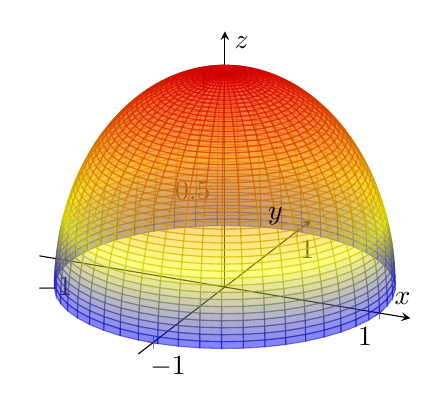
\begin{tikzpicture}
  \begin{axis}[width=.7\textwidth,
      samples=50,domain=0:360,y domain=0:90,
      xmin=-1.2,xmax=1.2,ymin=-1.2,ymax=1.2,zmin=0,zmax=1.2,
      xlabel={$x$},ylabel={$y$},zlabel={$z$},
    axis lines=center]
    \addplot3[surf,opacity=0.5]
    ({cos(x)*cos(y)}, {sin(x)*cos(y)}, {sin(y)});
  \end{axis}
\end{tikzpicture}

\begin{figure}[h]
	\centering
\begin{tikzpicture}[tdplot_main_coords, scale = 2.5]

% Create a point (P)
\coordinate (P) at ({1/sqrt(3)},{1/sqrt(3)},{1/sqrt(3)});

% Draw shaded circle
\shade[ball color = lightgray,
    opacity = 0.2
] (0,0,0) circle (1cm);

	\draw (0,-0.1,0) node {$0$};
	% \draw (0,-0.5,0) node {$D$};
	% \draw [-stealth] (-1/3, -1, 1) node[above left] {$z=\sqrt{R^2-x^2-y^2}$}
	% -- ({-1/sqrt(3)},{-1/sqrt(3)},{1/sqrt(3)});
	% \draw [-stealth] (1.5, -1, 0) node[above left] {$z=0$}
	-- (1,0,0);

% draw arcs
\tdplotsetrotatedcoords{0}{0}{0};
\draw[%dashed,
    tdplot_rotated_coords,
    gray, name path=dno,
	pattern=horizontal lines, pattern color=gray,
	opacity=1
] (0,0,0) circle (1);

% \tdplotsetrotatedcoords{90}{90}{90};
% \draw[dashed,
%     tdplot_rotated_coords,
%     gray
% ] (1,0,0) arc (0:180:1);

% \tdplotsetrotatedcoords{0}{90}{90};
% \draw[dashed,
%     tdplot_rotated_coords,
%     gray
% ] (1,0,0) arc (0:180:1);

% % Projection of the point on X and y axes
% \draw[thin, dashed] (P) --++ (0,0,{-1/sqrt(3)});
% \draw[thin, dashed] ({1/sqrt(3)},{1/sqrt(3)},0) --++
% (0,{-1/sqrt(3)},0);
% \draw[thin, dashed] ({1/sqrt(3)},{1/sqrt(3)},0) --++
% ({-1/sqrt(3)},0,0);

% Axes in 3 d coordinate system
\draw[-stealth] (0,0,0) -- (1.80,0,0)
    node[below left] {$x$};

\draw[-stealth] (0,0,0) -- (0,1.30,0)
    node[below right] {$y$};

\draw[-stealth] (0,0,0) -- (0,0,1.30)
    node[above] {$z$};

% \draw[dashed, gray] (0,0,0) -- (-1,0,0);
% \draw[dashed, gray] (0,0,0) -- (0,-1,0);

% Line from the origin to (P)
% \draw[thick, -stealth] (0,0,0) -- (P) node[right] {$P$};

% Add small circle at (P)
% \draw[fill = lightgray!50] (P) circle (0.5pt);

% \fill [
%        pattern={Lines[
%                   distance=2mm,
%                   angle=45,
%                   line width=0.7mm
%                  ]},
%         pattern color=blue
%        ] (0,0) rectangle (5,5);

\end{tikzpicture}
\caption{Область інтегрування}
\end{figure}

\begin{dmath}
	\iiint_V (x^2+y^2)\,dx\,dy\,dz,~V:x^2+y^2+z^2=R^2,~z\geq0
	% = \iint_D (x^2+y^2)\,dx\, dy \int_0^{\sqrt{R^2-x^2-y^2}} dz
	% = \iint_{G_{r\varphi}} r^2(1) \sqrt{R^2-1}
	% \,dr\,d\phi
% ...
	= \iiint_{W_{r\varphi\theta}}r^2\sin\theta
	\cdot r^2\sin^2\theta(\cos^2\phi+\sin^2\phi)
	\,dr\,d\phi\,d\theta
	= \iiint_{W_{r\varphi\theta}}r^4\sin^3\theta
	\,dr\,d\phi\,d\theta
\end{dmath}

\Answer{
	<++>
}

\end{document}
